\documentclass{article}
% PACKAGES
\usepackage[english]{babel}
\usepackage{graphicx} % Required for inserting images
\usepackage[most]{tcolorbox}
\usepackage{lmodern}
\usepackage{titlepic}
\usepackage{pdfpages}
\usepackage{tcolorbox}
\usepackage{amsmath}
\usepackage{pgfplots}
\usepackage{xcolor}
\usepackage{tikz}
\usepackage{color,soul}
\usepackage{enumerate}
\usepackage{enumitem}
\usepackage{cancel}
\usepackage{hyperref} 
\usepackage{tikzsymbols}
\usepackage{fontawesome5}
\usepackage[export]{adjustbox}
\usepackage{amssymb}
\usepackage{tikz,lipsum,lmodern}
\usepackage{booktabs}
\usepackage{tikz-3dplot}
\usepackage{tikz-cd}
\usepackage{circuitikz}

% COLOURS
\definecolor{Orchid}{RGB}{218, 112, 214}
\definecolor{snow}{rgb}{1.0, 0.98, 0.98}
\definecolor{mordantred19}{rgb}{0.68, 0.05, 0.0}
\definecolor{mistyrose}{rgb}{1.0, 0.89, 0.88}
\definecolor{nadeshikopink}{rgb}{0.96, 0.68, 0.78}
\definecolor{cadmiumgreen}{rgb}{0.0, 0.42, 0.24}
\definecolor{OliveGreen}{RGB}{85, 107, 47}
\definecolor{RoyalPurple}{RGB}{120, 81, 169}
\definecolor{NavyBlue}{RGB}{0, 0, 128}
\definecolor{CornflowerBlue}{RGB}{100, 149, 237}
\definecolor{Cerulean}{RGB}{0, 123, 167}
\definecolor{DarkOrchid}{RGB}{153, 50, 204}

\newcommand*\circled[1]{\tikz[baseline=(char.base)]{
            \node[shape=circle,draw,inner sep=2pt] (char) {#1};}}


\title{MCV4U - Calculus and Vectors [Chapter 7]}
\author{Kensukeken}
\date{May 10th, 2024}

\begin{document}
\maketitle

\tableofcontents
\newpage
\section{Unit 7 -  Applications of Vectors}
\subsection{Vectors in $R^2$ and $R^3$}
Any two-dimensional vector has a unique representation on the Cartesian plane in $R^2$.  The vector $\overrightarrow{OP}$ is a vector with its tail at the origin and its head at point $P(a,b)$. Different ways of expressing this vector include:
\begin{enumerate}
    \item[1.] $\overrightarrow{OP}$
    \item[2.](a,b)
    \item[3.] $\overrightarrow{(a,b)}$
\end{enumerate}
Similarly, any three-dimensional vector has a unique representation in $R^3$. The most common convention for expressing the x, y, and z-axes is the right-handed system of coordinates.  The vector $\overrightarrow{OP}$is a vector with its tail at the origin and its head at the point $P(a,b,c)$. Different ways of expressing this vector include:
\begin{enumerate}
    \item[1.] $\overrightarrow{OP}$
    \item[2.](a,b,c)
    \item[3.] $\overrightarrow{(a,b,c)}$
\end{enumerate}
\subsubsection*{Example 1} Using the right-handed system, sketch the vector $\overrightarrow{OP}$ where the coordinates of point P are (6,2,4).
\begin{center}
\centering
 \tdplotsetmaincoords{70}{110}
\begin{tikzpicture}[tdplot_main_coords]
  \draw[->] (0,0,0) -- (6,2,4) node[anchor=south]{$\overrightarrow{OP}$};
  \draw[dashed, color=gray] (0,0,0) -- (6,2,0) -- (6,2,4);
  \draw[dashed, color=gray] (6,2,0) -- (6,0,0);
  \draw[dashed, color=gray] (6,2,0) -- (0,2,0);
  \node at (7,2,4) {P(6,2,4)};
  \draw[thick,->] (0,0,0) -- (7,0,0) node[anchor=north east]{$x$};
  \draw[thick,->] (0,0,0) -- (0,3,0) node[anchor=north west]{$y$};
  \draw[thick,->] (0,0,0) -- (0,0,5) node[anchor=south]{$z$};
\end{tikzpicture}
\end{center}
\subsubsection*{Example 2} Using the right-handed system, sketch the vector $\overrightarrow{OP}$ where the coordinates of point P are (-2,1,-5).
\begin{center}
\centering
\tdplotsetmaincoords{70}{110}
\begin{tikzpicture}[tdplot_main_coords]
  \draw[->] (0,0,0) -- (-2,1,-5) node[anchor=north]{$\overrightarrow{OP}$};
  \draw[dashed, color=gray] (0,0,0) -- (-2,1,0) -- (-2,1,-5);
  \draw[dashed, color=gray] (-2,1,0) -- (-2,0,0);
  \draw[dashed, color=gray] (-2,1,0) -- (0,1,0);
  \node at (-3,1,-5) {P(-2,1,-5)};
  \draw[thick,->] (0,0,0) -- (-3,0,0) node[anchor=south east]{$x$};
  \draw[thick,->] (0,0,0) -- (0,2,0) node[anchor=south west]{$y$};
  \draw[thick,->] (0,0,0) -- (0,0,-6) node[anchor=east]{$z$};
\end{tikzpicture}
\end{center}

\subsection{Addition and Subtraction of Vectors in $R^2$ and $R^3$}

The unit vectors $\vec{\imath}, \vec{\jmath}$ and $\vec{k}$\\
Any vector in the two-dimensional plane can be expressed in terms of the unit vectors $\vec{\imath}$ and $\vec{\jmath}$ where $\vec{\imath}=\overrightarrow{(1,0)}$ and $\vec{\jmath}=\overrightarrow{(0,1)}$\\

For example, $\overrightarrow{(-3,4)}=-3 \overrightarrow{(1,0)}+4 \overrightarrow{(0,1)}=-3 \vec{\imath}+4 \vec{\jmath}$\\\\
Similarly, any vector in three dimensions can be expressed in terms of the unit vectors $\vec{\imath}, \vec{j}$ and $\vec{k}$ where $\vec{\imath}=\overrightarrow{(1,0,0}), \vec{j}=$ $\overrightarrow{(0,1,0)}$ and $\vec{k}=(0,0,1)$\\


For example, $\overrightarrow{(5,-2,-3)}=5 \overrightarrow{(1,0,0)}-2 \overrightarrow{(0,1,0)}-3 \overrightarrow{(0,0,1)}$
$$
=5 \vec{\imath}-2 \vec{\jmath}-3 \vec{k}
$$

\subsubsection{Distributive Property}
As a general rule, if $\vec{v}=\overrightarrow{(a, b)}$, then $k \vec{v}=k \overrightarrow{(a, b)}=\overrightarrow{(k a, k b)}$\\


For example, $5 \overrightarrow{(2,-3)}=\overrightarrow{(10,-15)}$\\



Similarly, if $\vec{v}=\overrightarrow{(a, b, c)}$, then $k \vec{v}=k \overrightarrow{(a, b, c)}=\overrightarrow{(k a, k b, k c)}$\\


For example, $-4 \overrightarrow{(6,-1,2)}=\overrightarrow{(-24,4,-8)}$\\

\subsubsection{Adding and Subtracting Vectors}


Given $\vec{a}=\overrightarrow{O A}=\overrightarrow{(1,3)}$ and $\vec{b}=\overrightarrow{O B}=(4,-2)$,

\subsubsection*{a) Graph $\overrightarrow{O A}$ and $\overrightarrow{O B}$}

\begin{center}
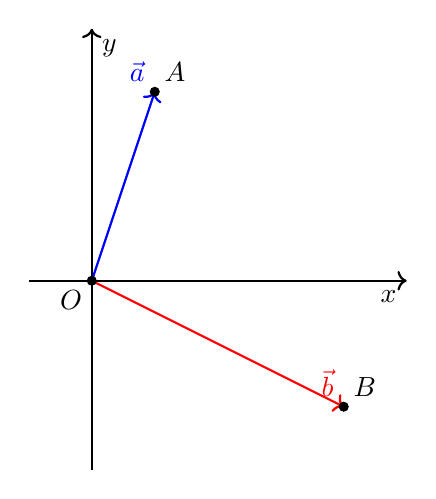
\begin{tikzpicture}[scale=0.8]
    % Axis
    \draw[thick,->] (-1,0) -- (5,0) node[anchor=north east]{$x$};
    \draw[thick,->] (0,-3) -- (0,4) node[anchor=north west]{$y$};
    % Vector a (OA)
    \draw[thick,->,blue] (0,0) -- (1,3) node[anchor=south east ]{$\vec{a}$};
    % Vector b (OB)
    \draw[thick,->,red] (0,0) -- (4,-2) node[anchor=south east]{$\vec{b}$};
    % Point O
    \filldraw[black] (0,0) circle (2pt) node[anchor=north east]{$O$};
    % Point A
    \filldraw[black] (1,3) circle (2pt) node[anchor=south west]{$A$};
    % Point B
    \filldraw[black] (4,-2) circle (2pt) node[anchor=south west]{$B$};
\end{tikzpicture}
\end{center}

\subsubsection*{b) Graph $\vec{a}+\vec{b}$ and state the components of that vector}

\begin{center}
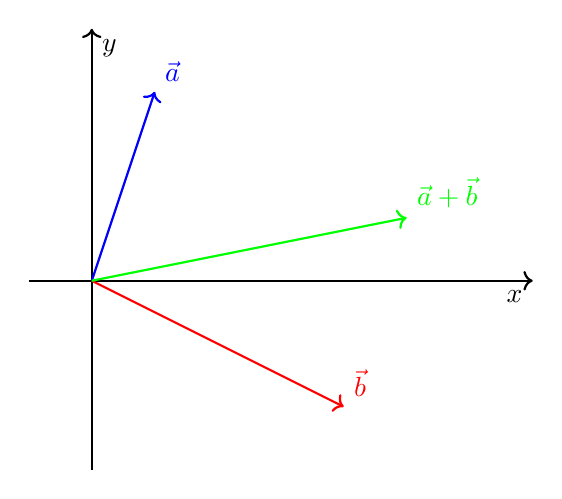
\begin{tikzpicture}[scale=0.8]
    % Axis
    \draw[thick,->] (-1,0) -- (7,0) node[anchor=north east]{$x$};
    \draw[thick,->] (0,-3) -- (0,4) node[anchor=north west]{$y$};
    % Vector a (OA)
    \draw[thick,->,blue] (0,0) -- (1,3) node[anchor=south west]{$\vec{a}$};
    % Vector b (OB)
    \draw[thick,->,red] (0,0) -- (4,-2) node[anchor=south west]{$\vec{b}$};
    % Vector a+b
    \draw[thick,->,green] (0,0) -- (5,1) node[anchor=south west]{$\vec{a}+\vec{b}$};
\end{tikzpicture}
\end{center}

Components of $\vec{a}+\vec{b}$: $(1+4, 3+(-2)) = (5, 1)$

\subsubsection*{c) Graph $\vec{a}-\vec{b}$ and state the components of that vector}

\begin{center}
\begin{tikzpicture}[scale=0.8]
    % Axis
    \draw[thick,->] (-1,0) -- (7,0) node[anchor=north east]{$x$};
    \draw[thick,->] (0,-3) -- (0,4) node[anchor=north west]{$y$};
    % Vector a (OA)
    \draw[thick,->,blue] (0,0) -- (1,3) node[anchor=south west]{$\vec{a}$};
    % Vector b (OB)
    \draw[thick,->,red] (0,0) -- (4,-2) node[anchor=south west]{$\vec{b}$};
    % Vector a-b
    \draw[thick,->,purple] (0,0) -- (-3,5) node[anchor=south west]{$\vec{a}-\vec{b}$};
\end{tikzpicture}
\end{center}

Components of $\vec{a}-\vec{b}$: $(1-4, 3-(-2)) = (-3, 5)$
\begin{tcolorbox}[enhanced,frame style image=blueshade.png,
  opacityback=0.75,opacitybacktitle=0.25,
  colback=blue!5!white,colframe=blue!75!black]
In short, if $\vec{a}=\overrightarrow{\left(x_1, y_1\right)}$ and if $\vec{b}=\overrightarrow{\left(x_2, y_2\right)}$, then
$$
\vec{a}+\vec{b}=\overrightarrow{\left(x_1+x_2, y_1+y_2\right)}
$$

This also works in 3 dimensions. In other words, if\\
$\vec{a}=\overrightarrow{(x_1,y_1,z_1)}$ and if $\vec{b}=\overrightarrow{(x_2,y_2,z_2)}$, then 
$$\vec{a}+\vec{b}=\overrightarrow{(x_1+x_2,y_1+y_2,z_1+z_2)}$$
\end{tcolorbox}

\subsubsection{Subtracting vectors} Notice that if we are to subtract vector $\vec{b}$ from vector $\vec{a}$, we can do so by the tip-to-tail meth well.

We add the opposite of $\vec{b}$ to $\vec{a}$. In other words, $\vec{a}-\vec{b}=\vec{a}+(-\vec{b})$
So, for example,
$$
\overrightarrow{(1,3)}-\overrightarrow{(4,-2)}=\overrightarrow{(-3,5)}
$$
\begin{tcolorbox}[enhanced,frame style image=blueshade.png,
  opacityback=0.75,opacitybacktitle=0.25,
  colback=blue!5!white,colframe=purple!75!black]
In short, if $\vec{a}=\overrightarrow{\left(x_1, y_1\right)}$ and if $\vec{b}=\overrightarrow{\left(x_2, y_2\right)}$, then
$$
\vec{a}-\vec{b}=\overrightarrow{\left(x_1-x_2, y_1-y_2\right)}
$$

This also works in 3 dimensions. In other words, if $\vec{a}=\overrightarrow{\left(x_1, y_1, z_1\right)}$ and if $\vec{b}=\overrightarrow{\left(x_2, y_2, z_2\right)}$, then
$$
\vec{a}-\vec{b}=\overrightarrow{\left(x_1-x_2, y_1-y_2, z_1-z_2\right)}
$$
\end{tcolorbox}
\subsubsection{Magnitudes of Vectors}
\begin{tcolorbox}[enhanced,frame style image=blueshade.png,
  opacityback=0.75,opacitybacktitle=0.25,
  colback=blue!5!white,colframe=purple!75!black]
-Given the points $A\left(x_1, y_1\right)$ and $B\left(x_2, y_2\right)$,
$\overrightarrow{A B}=\overrightarrow{\left(x_2-x_1, y_2-y_1\right)}$ and $|\overrightarrow{A B}|=\sqrt{\left(x_2-x_1\right)^2+\left(y_2-y_1\right)^2}$
Similarly, given the points $A\left(x_1, y_1, z_1\right)$ and $B\left(x_2, y_2, z_2\right)$,
$$
\begin{aligned}
\overrightarrow{A B}=\overrightarrow{\left(x_2-x_1, y_2-y_1, z_2-z_1\right)} \text { and } \\
|\overrightarrow{A B}|=\sqrt{\left(x_2-x_1\right)^2+\left(y_2-y_1\right)^2+\left(z_2-z_1\right)^2}
\end{aligned}
$$
\end{tcolorbox}
\subsubsection{Example 1}
Determine $\overrightarrow{A B}$ and $|\overrightarrow{A B}|$ where the coordinates of $\mathrm{A}$ are $(3,2,-5)$ and the coordinates of $\mathrm{B}$ are $(-4,0,-3)$.
\begin{align*}
    \overrightarrow{AB}&=(-4-3,0-2,-3-(-5))\\
    &\boxed{\overrightarrow{AB}=(-7,-2,2)}\\
    |\overrightarrow{AB}| &=\sqrt{(-7)^2+(-2)^2+(2)^2}\\
    &=\sqrt{49+4+4}\\
    &=\sqrt{57}
\end{align*}
\newpage
\subsubsection{Example 2}
For the vector shown at the right determine the components of the position vector. 

\vspace{2em}
\begin{minipage}{0.5\textwidth}
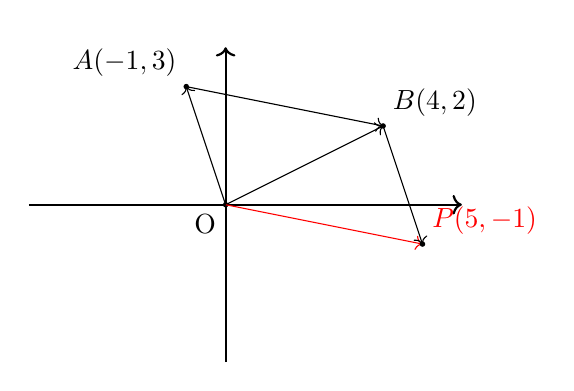
\begin{tikzpicture}[scale=0.5]
    % Draw axes
    \draw[thick, ->] (-5, 0) -- (6, 0) node[anchor=north west] {};
    \draw[thick, ->] (0, -4) -- (0, 4) node[anchor=south east] {};
    \fill (0,0) circle (2pt) node[below left] {O};

    
    % Draw points and arrows
    \draw[->] (0,0) -- (4,2) node[anchor=south west] {$B(4,2)$};
    \draw[->,red] (0,0) -- (5,-1) node[anchor=south west] {$P(5,-1)$};
    \draw[->] (0,0) -- (-1,3) node[anchor=south east] {$A(-1,3)$};
    
    % Draw connections between points
    \draw[->] (-1,3) -- (4,2);
    \draw[->] (4,2) -- (5,-1);
    
    % Draw points
    \fill (4,2) circle (2pt);
    \fill (5,-1) circle (2pt);
    \fill (-1,3) circle (2pt);
\end{tikzpicture}
\end{minipage}
\begin{minipage}{0.5\textwidth}
$$\overrightarrow{OP}=(4-(-1),2-3)$$
$$=(5,-1)$$
\end{minipage}

\subsubsection{Example 2}
Parallelogram OABC is determined by the vectors $\overrightarrow{OA}=\overrightarrow{7,4}$ and $\overrightarrow{OC}=\overrightarrow{(1,-6)}$.
Determine $\overrightarrow{OB},\overrightarrow{AB}$ and $\overrightarrow{BC}$

\subsubsection*{Solution}
\begin{minipage}{0.5\textwidth}
Given: $\overrightarrow{OA} = \begin{pmatrix} 7 \\ 4 \end{pmatrix}$ and $\overrightarrow{OC} = \begin{pmatrix} 1 \\ -6 \end{pmatrix}$.

\begin{center}
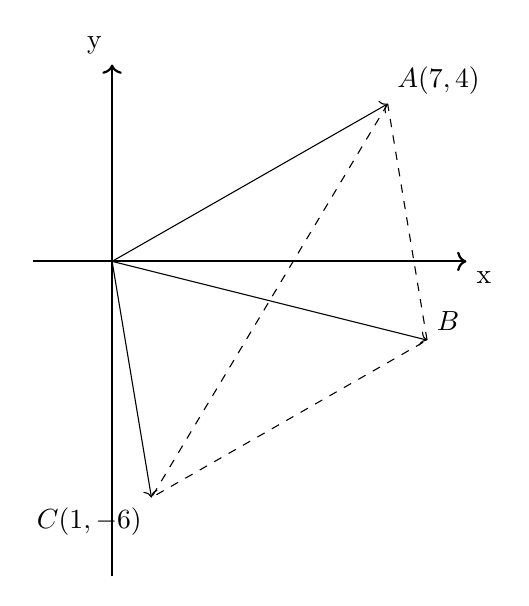
\begin{tikzpicture}[scale=0.5]
    % Draw axes
    \draw[thick, ->] (-2,0) -- (9,0) node[anchor=north west] {x};
    \draw[thick, ->] (0,-8) -- (0,5) node[anchor=south east] {y};
    
    % Draw points and vectors
    \coordinate (A) at (7,4);
    \coordinate (C) at (1,-6);
    \coordinate (B) at ($(A)+(C)$);
    
    \draw[->] (0,0) -- (A) node[anchor=south west] {$A(7,4)$};
    \draw[->] (0,0) -- (C) node[anchor=north east] {$C(1,-6)$};
    \draw[->] (0,0) -- (B) node[anchor=south west] {$B$};
    
    % Draw the parallelogram
    \draw[dashed] (A) -- node[midway, left] {} (C) -- node[midway, below] {} (B);
    \draw[dashed] (B) -- node[midway, right] {} (A);
\end{tikzpicture}
\end{center}
\end{minipage}
\begin{minipage}{0.5\textwidth}
\subsubsection*{Solution}
\begin{align*}
\overrightarrow{OB} &= \overrightarrow{OA} + \overrightarrow{OC} = \begin{pmatrix} 7 \\ 4 \end{pmatrix} + \begin{pmatrix} 1 \\ -6 \end{pmatrix} = \begin{pmatrix} 8 \\ -2 \end{pmatrix} \\
\overrightarrow{AB} &= \overrightarrow{OB} - \overrightarrow{OA} = \begin{pmatrix} 8 \\ -2 \end{pmatrix} - \begin{pmatrix} 7 \\ 4 \end{pmatrix} = \begin{pmatrix} 1 \\ -6 \end{pmatrix} \\
\overrightarrow{BC} &= \overrightarrow{OC} - \overrightarrow{OA} = \begin{pmatrix} 1 \\ -6 \end{pmatrix} - \begin{pmatrix} 7 \\ 4 \end{pmatrix} = \begin{pmatrix} -6 \\ -10 \end{pmatrix}
\end{align*}
\end{minipage}

\subsubsection*{Example 3}
If $\vec{u}=-2\vec{i}+6\vec{k}$, and if $\vec{v}=\vec{i}-\vec{j}+\vec{k}$, determine $3\vec{u}-2\vec{v}$ and $|3\vec{u}-2\vec{v}|$.
\subsubsection*{Solution}
\begin{minipage}{0.5\textwidth}
\begin{align*}
\vec{u}&=-2\vec{j}+9\vec{j}+6\vec{k}\\
&=(-2,9,6)\\
\vec{v}&=\vec{i}-\vec{j}+\vec{k}\\
&=\overrightarrow{(1,-1,1)}
\end{align*}
\end{minipage}
\begin{minipage}{0.5\textwidth}
\begin{align*}
3\vec{u}-2\vec{v}&=3\overrightarrow{(-2,9,6)}-2\overrightarrow{(1,-1,1)}\\
    &=\overrightarrow{(-6-2,27+2,18-2)}\\
    &=(-8,29,16)\\
    |3\vec{u}-2\vec{v}|&=\sqrt{(-8)^2+(29)^2+(16)^2}\\
    &=\sqrt{1161}
\end{align*}
\end{minipage}
\subsubsection*{Example 4}
A parallelogram is formed by the vectors $\overrightarrow{OA}=\begin{pmatrix} 3 \\ -1 \\ 4 \end{pmatrix}$, $\overrightarrow{OB}=\begin{pmatrix} -1 \\ 8 \\ -7 \end{pmatrix}$, and $\overrightarrow{OC}=\begin{pmatrix} 4 \\ 0 \\ -9 \end{pmatrix}$. Determine the coordinates of all the vertices for the parallelepiped.
\subsubsection*{Solution}
The coordinates of the vertices are:
\begin{align*}
A &= (3, -1, 4) \\
B &= A + \overrightarrow{OB} = (3, -1, 4) + (-1, 8, -7) = (2, 7, -3) \\
C &= A + \overrightarrow{OC} = (3, -1, 4) + (4, 0, -9) = (7, -1, -5) \\
D &= B + \overrightarrow{OC} = (2, 7, -3) + (4, 0, -9) = (6, 7, -12)
\end{align*}

\subsubsection*{Example 5}
Determine the midpoint of the points $A(-4,3,9)$ and $B(2,-11,7)$.
\subsubsection*{Solution}
The midpoint of two points is calculated by taking the average of their coordinates. Therefore, the midpoint of $A$ and $B$ is:
\begin{align*}
\text{Midpoint}
&= \left(\frac{x_1+x_2}{2}, \frac{y_1+y_2}{2}, \frac{z_1+z_2}{2}\right) \\
&= \left(\frac{-4+2}{2}, \frac{3+(-11)}{2}, \frac{9+7}{2}\right) \\
&= (-1, -4, 8)
\end{align*}
\newpage 
\subsection{Linear Combinations and Spanning Sets}
A set of two vectors forms a spanning set for \(\mathbb{R}^2\) if every vector in \(\mathbb{R}^2\) can be written as a linear combination of those two vectors.\\\\
If \(\vec{u}\), \(\vec{v}\), and \(\vec{w}\) are vectors and if \(\vec{w} = a\vec{u} + b\vec{v}\) where \(a\) and \(b\) are scalars, then \(\vec{w}\) can be written as a linear combination of \(\vec{u}\) and \(\vec{v}\).\\\\
For example, the vectors \(\vec{i}\) and \(\vec{j}\) span \(\mathbb{R}^2\) because every vector in \(\mathbb{R}^2\) can be written as a linear combination of \(\vec{i}\) and \(\vec{j}\). To illustrate:
\[\overrightarrow{(4,-3)} = 4\vec{i} - 3\vec{j}\]
\subsubsection{Example 1}
Show that \(\vec{v}=\overrightarrow{(4,23)}\) can be written as a linear combination of the set of vectors \(\{\overrightarrow{(-1,4)},\overrightarrow{(2,5)}\}\)
\subsubsection*{Solution}
In other words, we want to show that we can get from the origin to the point (4, 23) using only the two vectors shown\\

\begin{minipage}{0.5\textwidth}
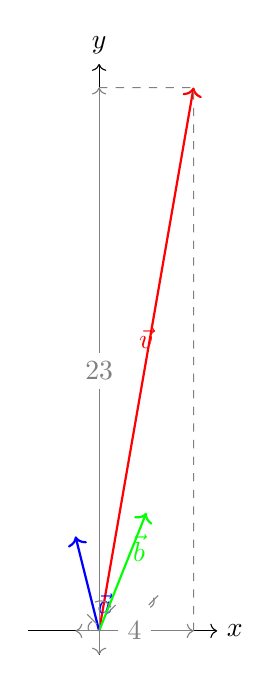
\begin{tikzpicture}[scale=0.3]
% Define the vectors
\coordinate (origin) at (0,0);
\coordinate (v) at (4,23);
\coordinate (a) at (-1,4);
\coordinate (b) at (2,5);

% Draw the axes
\draw[->] (-3,0) -- (5,0) node[right] {$x$};
\draw[->] (0,-1) -- (0,24) node[above] {$y$};

% Draw the vectors
\draw[->,red,thick] (origin) -- (v) node[midway,above] {$\vec{v}$};
\draw[->,blue,thick] (origin) -- (a) node[midway,below right] {$\vec{a}$};
\draw[->,green,thick] (origin) -- (b) node[midway,above right] {$\vec{b}$};

% Draw the components of v
\draw[dashed,gray] (4,0) -- (v);
\draw[dashed,gray] (0,23) -- (v);

% Label the components of v
\draw[<->,gray] (0,-1) -- node[fill=white] {$23$} (0,23);
\draw[<->,gray] (-1,0) -- node[fill=white] {$4$} (4,0);

% Add a right angle symbol for clarity
\draw[gray] (0.5,1) arc (26.57:116.57:0.5);
\draw[gray] (0.3,0.7) -- (0.7,1.1);

% Add a right angle symbol for vector a
\draw[gray] (-0.3,0.4) arc (116.57:206.57:0.3);
\draw[gray] (-0.5,0.7) -- (-0.1,0.3);

% Add a right angle symbol for vector b
\draw[gray] (2.3,1.4) arc (26.57:-63.43:0.3);
\draw[gray] (2.1,1.1) -- (2.5,1.5);

\end{tikzpicture}
\end{minipage}
\begin{minipage}{0.5\textwidth}
\begin{align*}
\overrightarrow{(4,23)}&=a\overrightarrow{(-1,4)}+b\overrightarrow{(2,5)}\\
4&=-a+2b\\
23&=4a+5b\\
a&=2b-4\\
23&=4(2b-4)+56\\
23&=8b-16+56\\
39&=13b\\
b&=3\\
a&=2b-4 \implies a=2(3)-4\\
a&=2
\end{align*}
\end{minipage}
$$\therefore \overrightarrow{(4,23)}=2\overrightarrow{(-1,4)}+3\overrightarrow{(2,5)}$$

\subsubsection{Term to Know: Spanning Set} 
A spanning set of $\mathbb{R}^2$ exists if every vector in $\mathbb{R}^2$ can be written as a linear combination of those vectors.
\[\{\overrightarrow{(1,0)}, \overrightarrow{(0,1)}\}\]

\subsubsection*{Example 2}
Show that the set of vectors \(\{\overrightarrow{(2,3)}, \overrightarrow{(-4,-6)}\}\) is not a spanning set of $\mathbb{R}^2$
\subsubsection*{Solution}
Try an counter example. We'll try $(3,2)$.\\
Let $\overrightarrow{(3,2)}=a\overrightarrow{(2,3)}+b\overrightarrow{(-4,-6)}$\\
\begin{minipage}[t]{0.5\textwidth}
\begin{align*}
    \therefore 3&=2a-4b\\
    2&=3a-6b\\
\end{align*}    
\end{minipage}
\begin{minipage}[t]{0.5\textwidth}
\text{Using elimination}
$$
\begin{array}{ccccc}
    9&=6a-12b \quad \text{(1) $\times$ 3}\\
    4&=6a-12b \quad \text{(2) $\times$ 2}\\
    \hline\\
    5&=0a+0 \quad \text{Not possible} 
\end{array}
$$    
\end{minipage}
\\\\
$\therefore \overrightarrow{(3,2)}$ is not a linear combination of $\overrightarrow{(2,3)}$ and $\overrightarrow{(-4,-6)}$.\\
$\therefore \{\overrightarrow{(2,3)}, \overrightarrow{(-4,-6)}\}$ is not a spanning set of $\mathbb{R}^2$.

\subsubsection{Terms to Know: Collinear Vectors}
Two vectors are collinear vectors if they are parallel and lie on the same straight line. We can tell algebraically if two vectors are collinear by determining whether they are scalar multiples of each other.

Examples:
1. $\overrightarrow{(-3,2)}$ and $\overrightarrow{(12,-8)}$ are collinear.
2. $\overrightarrow{(5,15,-30)}$ and $\overrightarrow{(1,3,-6)}$ are collinear.
3. $\overrightarrow{(9,4)}$ and $\overrightarrow{(3,2)}$ are not collinear.
4. $\overrightarrow{(-8,-12,4)}$ and $\overrightarrow{(2,-3,-1)}$ are not collinear.
\begin{tcolorbox}[enhanced,frame style image=blueshade.png,
  opacityback=0.75,opacitybacktitle=0.25,
  colback=blue!5!white,colframe=blue!75!black]
  \begin{itemize}
      \item General Rule Regarding Spanning Sets
      \item Any two non-zero, non-collinear vectors in $R^2$ span $R^2$.
\item Any two collinear vectors in $R^2$ do not span $R^2$.
  \end{itemize}
\end{tcolorbox}
\begin{tcolorbox}[enhanced,frame style image=blueshade.png,
  opacityback=0.75,opacitybacktitle=0.25,
  colback=blue!5!white,colframe=blue!75!black] 
  \begin{itemize}
      \item Another Similar and Related Rule Regarding Spanning Sets
\item Any two non-zero, non-collinear vectors in $R^3$ span a plane (two-dimensional) in $R^3$. This means that there will be many other vectors in $R^3$ on that plane and many other vectors in $R^3$ not on that plane.
\item As an example, think of the vectors $\vec{\imath}=\overrightarrow{(1,0,0)}$ and $\vec{\jmath}=\overrightarrow{(0,1,0)}$. These vectors are not collinear, yet they span the entire plane consisting of all vectors with a z-component of 0 . (we will talk in great detail later in the course about the equations of planes)
\item 
Any two collinear vectors in $R^3$ do not span a plane in $R^3$.
  \end{itemize}
\end{tcolorbox}

\subsubsection{Example 1}
Give the two vectors $\vec{a}=\overrightarrow{(-1,-2,1)}$ and $\vec{b}=\overrightarrow{(3,-1,1)}$, does the vector $\vec{c}=\overrightarrow{(-9,-4,1)}$ lie on the plane spanned by $\vec{a}$ and $\vec{b}$?
\subsubsection*{Solution}
 if vector $\vec{c}$ lies on the plane spanned by $\vec{a}$ and $\vec{b}$, we can check if $\vec{c}$ can be expressed as a linear combination of $\vec{a}$ and $\vec{b}$. That is, we need to find scalars $x$ and $y$ such that:
\[
\vec{c} = x\vec{a} + y\vec{b}
\]
Substituting the given vectors into the equation, we get:
\[
\overrightarrow{(-9,-4,1)} = x\overrightarrow{(-1,-2,1)} + y\overrightarrow{(3,-1,1)}
\]
This gives us the system of equations:

\begin{align*}
-9 &= -x + 3y \\
-4 &= -2x - y \\
1 &= x + y
\end{align*}

Solving this system, we find that $x = 2$ and $y = -1$ satisfy all three equations. Therefore, $\vec{c}$ does lie on the plane spanned by $\vec{a}$ and $\vec{b}$.


\subsubsection{Example 2}
Give the two vectors $\vec{a}=\overrightarrow{(-1,-2,1)}$ and $\vec{b}=\overrightarrow{(3,-1,1)}$, does the vector $\vec{c}=\overrightarrow{(-9,-4,2)}$ lie on the plane spanned by $\vec{a}$ and $\vec{b}$?
\subsubsection*{Solution }
Using the same approach, we set up the equation:
\[
\overrightarrow{(-9,-4,2)} = x\overrightarrow{(-1,-2,1)} + y\overrightarrow{(3,-1,1)}
\]
Which leads to the system:

\begin{align*}
-9 &= -x + 3y \\
-4 &= -2x - y \\
2 &= x + y
\end{align*}

However, this system does not have a solution where $x$ and $y$ satisfy all three equations simultaneously. Therefore, $\vec{c}$ does not lie on the plane spanned by $\vec{a}$ and $\vec{b}$.

\subsection{Dot Product(Aka Scalar Product)}
The dot product of the vectors $\vec{a}$ and $\vec{b}$ is equal to magnitude of $\vec{a}$ times the magnitude of $\vec{b}$ times the cosine of the angle between them.\\\\
In other words,
\[\vec{a}\cdot \vec{b}=|\vec{a}||\vec{b}|\cos \theta\]

\subsubsection*{Example 1}
Give the magnitude of $\vec{a}$ is 7, the magnitude of $\vec{b}$ is 4, and that there is an angle of $60^{\circ}$ between $\vec{a}$ and $\vec{b}$, evaluate $\vec{a}\cdot \vec{b}$

\subsubsection*{Solution}
$$\vec{a}\cdot \vec{b}=(7)(4)\cos 60^{\circ}\implies 14$$
\subsubsection*{Example 2}
Give the magnitude of $\vec{a}$ is 9, the magnitude of $\vec{b}$ is 5, and that there is an angle of $140^{\circ}$ between $\vec{a}$ and $\vec{b}$, evaluate $\vec{a}\cdot \vec{b}$

\subsubsection*{Solution}
$$\vec{a}\cdot \vec{b}=(9)(5)\cos 140^{\circ}\implies -34.5$$
That's it :)
\newpage 

\subsubsection{$\underline{R e l a t i o n s h i p ~ B e t w e e n ~ D o t ~ P r o d u c t ~ a n d ~ A n g l e ~ B e t w e e n ~ V e c t o r s ~}$}
Assume that neither $\vec{a}$ nor $\vec{b}$ have a magnitude of 0 , meaning that each of the magnitudes is positive.
Next, recall the following:\\
\begin{enumerate}
    \item $\cos \theta>0$ if $0^0 \leq \theta<90^{\circ}$
    \item $\cos \theta=0$ if $\theta=90^{\circ}$
    \item $\cos \theta<0$ if $90^{\circ}<\theta \leq 180^{\circ}$
\end{enumerate}


Since $\vec{a} \cdot \vec{b}=|\vec{a}||\vec{b}| \cos \theta$, therefore:\\
\begin{tcolorbox}[enhanced,frame style image=blueshade.png,
  opacityback=0.75,opacitybacktitle=0.25,
  colback=blue!5!white,colframe=blue!75!black] 
\begin{enumerate}
    \item $\vec{a} \cdot \vec{b}$ is positive if $\theta$ is acute
    \item $\vec{a} \cdot \vec{b}=0$ if $\theta=90^{\circ}$
    \item $\vec{a} \cdot \vec{b}$ is negative if $\theta$ is obtuse
\end{enumerate}

* A significant detail of this course is that two vectors are perpendicular if and only if the dot product is 0
\end{tcolorbox}
\subsubsection*{Example 3}
Determine the value of $\vec{a} \cdot \vec{a}$ given that $|\vec{a}|=7$
\subsubsection*{Solution}
\begin{align*}
    \vec{a}\cdot \vec{b}&=|\vec{a}||\vec{b}|\cos \theta\\
    &=(7)(7)\cos \theta\\
    &=49\\
    &=|\vec{a}|
\end{align*}
\subsubsection{Properties of the Dot Product}
\textcolor{blue}{\textbf{Commutative Property:}}
\[
\vec{a} \cdot \vec{b}=\vec{b} \cdot \vec{a}
\]

\textcolor{blue}{\textbf{Associative Property:}}
\[
(m \vec{a}) \cdot \vec{b}=m(\vec{a} \cdot \vec{b}) \quad \text{For example, } (3 \vec{a}) \cdot \vec{b}=3(\vec{a} \cdot \vec{b})
\]

\textcolor{blue}{\textbf{Distributive Property (2):}}
\[
\begin{aligned}
& \vec{a} \cdot(\vec{b}+\vec{c})=\vec{a} \cdot \vec{b}+\vec{a} \cdot \vec{c} \\
& (\vec{a}+\vec{b}) \cdot(\vec{c}+\vec{d})=\vec{a} \cdot \vec{c}+\vec{a} \cdot \vec{d}+\vec{b} \cdot \vec{c}+\vec{b} \cdot \vec{d}
\end{aligned}
\]

\subsubsection*{Example 4}
Suppose the vectors $\vec{a}+3 \vec{b}$ and $4 \vec{a}-\vec{b}$ are perpendicular and suppose that $|\vec{a}|=2|\vec{b}|$. Determine the angle between the vectors $\vec{a}$ and $\vec{b}$.

\subsubsection*{Solution}
\begin{align*}
    (\vec{a}+3\vec{b})\cdot (4\vec{a}+\vec{b})&=0\\
    4\vec{a}\cdot \vec{a} -\vec{a}\cdot \vec{b}+12\vec{a} \cdot \vec{b}-3\vec{b}\cdot \vec{b}&=0\\
    4|\vec{a}|^2+11\vec{a}\cdot \vec{b}-3|\vec{b}|^2&=0\\
    4(2|\vec{b}|)^2+11\vec{a}\cdot \vec{b}-3|\vec{b}|^2&=0\\
    4(4|\vec{b}|^2)+11\vec{a}\cdot \vec{b}-3|\vec{b}|^2&=0\\
    16|\vec{b}|^2+11\vec{a} \cdot \vec{b}-3|\vec{b}|^2&=0\\
    13|\vec{b}|^2+11\vec{a}\cdot \vec{b}&=0\\
    13|\vec{b}|^2+11|\vec{a}||\vec{b}|\cos \theta&=0\\
    13|\vec{b}|^2+11[2|\vec{b}|]|\vec{b}|\cos\theta&=0\\
    13|\vec{b}|^2+22|\vec{b}|^2\cos \theta&=0\\
    22 \cdot |\vec{b}|\cos \theta&=-13|\vec{b}|^2\\
    \cos\theta &= \frac{-13|\vec{b}|^2}{22|\vec{b}|^2}\\
    \theta&=126.2^{\circ} 
\end{align*}
Therefore, the angle between $\vec{a}$ and $\vec{b}$ is approximately $126.2^{\circ}$

\subsubsection*{Example 5}
If $|\vec{x}+\vec{y}|=|\vec{x}-\vec{y}|$, then prove that the non-zero vectors $\vec{x}$ and $\vec{y}$ are perpendicular.
\subsubsection*{Solution}
\begin{align*}
    |\vec{x}+\vec{y}|^2&=|\vec{x}-\vec{y}|^2\\
    (\vec{x}+\vec{y})\cdot(\vec{x}+\vec{y})&=(\vec{x}-\vec{y})\\
    \cancel{\vec{x}\cdot\vec{x}}+2\vec{x}\cdot +\cancel{\vec{y}\cdot \vec{y}}&=\vec{x}\cdot \vec{x}-2\vec{x}\cdot \vec{y}+\cancel{\vec{y}\cdot \vec{y}}\\
    4\vec{x}\cdot \vec{y}&=0\\
    \vec{x} \cdot \vec{y}&=0\\
    \therefore &\vec{x} \text{ and } \vec{y} \text{are perpendicular}
\end{align*}

\subsection{Dot product Component Method}
\begin{tcolorbox}[enhanced,frame style image=blueshade.png,
  opacityback=0.75,opacitybacktitle=0.25,
  colback=blue!5!white,colframe=blue!75!black] 
  \begin{itemize}
      \item In $R^2$, given that $\vec{a}=\overrightarrow{\left(a_1, a_2\right)}$ and that $\vec{b}=\overrightarrow{\left(b_1, b_2\right)}$, then
$$
\vec{a} \cdot \vec{b}=a_1 b_1+a_2 b_2
$$
\item In $R^3$, given that $\vec{a}=\overrightarrow{\left(a_1, a_2, a_3\right)}$ and that $\vec{b}=\overrightarrow{\left(b_1, b_2, b_3\right)}$, then $\vec{a} \cdot \vec{b}=a_1 b_1+a_2 b_2+a_3 b_3$
\end{itemize}
\end{tcolorbox}

\subsubsection*{Example 1}
Determine the angle between the vectors $\vec{a}=\overrightarrow{(1,-3,4)}$ and $\vec{b}=\overrightarrow{(-8,5,7)}$.

\subsubsection*{Solution}
The angle $\theta$ between two vectors $\vec{a}$ and $\vec{b}$ is given by:
\[ \cos \theta = \frac{\vec{a} \cdot \vec{b}}{\|\vec{a}\| \|\vec{b}\|} \]

Where $\vec{a} \cdot \vec{b}$ is the dot product of vectors $\vec{a}$ and $\vec{b}$, and $\|\vec{a}\|$ and $\|\vec{b}\|$ are the magnitudes of vectors $\vec{a}$ and $\vec{b}$ respectively.

Given vectors:
\[ \vec{a} = \langle 1, -3, 4 \rangle \]
\[ \vec{b} = \langle -8, 5, 7 \rangle \]

The dot product $\vec{a} \cdot \vec{b}$ is:
\[ \vec{a} \cdot \vec{b} = (1)(-8) + (-3)(5) + (4)(7) = -8 - 15 + 28 = 5 \]

The magnitudes of vectors $\vec{a}$ and $\vec{b}$ are:
\[ \|\vec{a}\| = \sqrt{1^2 + (-3)^2 + 4^2} = \sqrt{1 + 9 + 16} = \sqrt{26} \]
\[ \|\vec{b}\| = \sqrt{(-8)^2 + 5^2 + 7^2} = \sqrt{64 + 25 + 49} = \sqrt{138} \]

So, the cosine of the angle between the vectors is:
\[ \cos \theta = \frac{5}{\sqrt{26} \cdot \sqrt{138}} \]

Therefore, the angle $\theta$ is:
\[ \theta = \arccos \left( \frac{5}{\sqrt{26} \cdot \sqrt{138}} \right) \implies \theta \approx 85.2^{\circ} \]

\subsubsection*{Example 2}
For what value(s) of $k$ are the vectors $\overrightarrow{(-1,3,4)}$ and $\overrightarrow{(3,k,-2)}$ perpendicular.

\subsubsection*{Solution}
Two vectors are perpendicular if their dot product is zero.

Given vectors:
\[ \vec{a} = \langle -1, 3, 4 \rangle \]
\[ \vec{b} = \langle 3, k, -2 \rangle \]

The dot product $\vec{a} \cdot \vec{b}$ is:
\[ \vec{a} \cdot \vec{b} = (-1)(3) + (3)(k) + (4)(-2) = -3 + 3k - 8 = 3k - 11 \]

For the vectors to be perpendicular, $\vec{a} \cdot \vec{b}$ must be zero:
\[ 3k - 11 = 0 \]
\[ 3k = 11 \]
\[ k = \frac{11}{3} \]

So, for the vectors to be perpendicular, $k$ must be $\frac{11}{3}$.

\subsubsection*{Example 3}
Determine the acute and obtuse angles between the diagonals of a box that measures 12 cm by 4 cm by 6 cm
\usetikzlibrary{calc}

\begin{center}

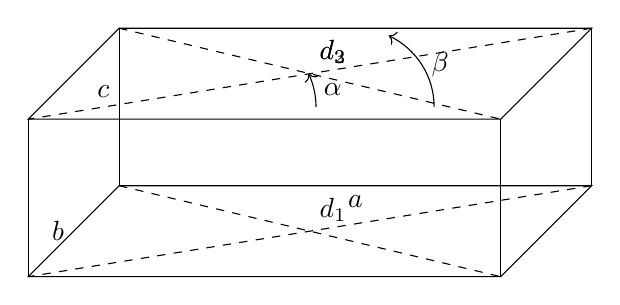
\begin{tikzpicture}[scale=0.5]
% Define vertices
\coordinate (A) at (0,0,0);
\coordinate (B) at (12,0,0);
\coordinate (C) at (12,0,6);
\coordinate (D) at (0,0,6);
\coordinate (E) at (0,4,0);
\coordinate (F) at (12,4,0);
\coordinate (G) at (12,4,6);
\coordinate (H) at (0,4,6);

% Draw edges
\draw (A) -- (B) -- (C) -- (D) -- cycle;
\draw (A) -- (E);
\draw (B) -- (F);
\draw (C) -- (G);
\draw (D) -- (H);
\draw (E) -- (F) -- (G) -- (H) -- cycle;

% Draw diagonals
\draw[dashed] (A) -- (C);
\draw[dashed] (B) -- (D);
\draw[dashed] (E) -- (G);
\draw[dashed] (F) -- (H);

% Add labels
\node at ($(A)!0.5!(B)$) [below] {$a$};
\node at ($(A)!0.5!(D)$) [left] {$b$};
\node at ($(A)!0.5!(E)$) [above left] {$c$};

% Show diagonals
\node at ($(A)!0.5!(C)$) [above right] {$d_1$};
\node at ($(E)!0.5!(G)$) [above right] {$d_2$};
\node at ($(F)!0.5!(H)$) [above right] {$d_3$};

% Draw angles
\draw[->] (5,2,0) arc (0:25:2) node[midway, right] {$\alpha$};
\draw[->] (8,2,0) arc (0:65:2) node[midway, right] {$\beta$};

\end{tikzpicture}
\end{center}
\subsection*{Solution}
\begin{align*}
    \vec{d_1}&=\overrightarrow{(12,4,6)} \quad \vec{d_2}=\overrightarrow{(12,4,6)}\\
    \vec{d_1}\cdot \vec{d_2}&=|\vec{d_1}||\vec{d_2}|\cos\theta\\
    144-16+36&=\sqrt{196}\sqrt{196}\cos \theta\\
    \frac{164}{\sqrt{196}\sqrt{196}}&=\cos \theta\\
    \theta \approx 33.2^{\circ} 
\end{align*}

\newpage 

\subsection{Scalar and Vector Projections}
Refer to diagram below
\[\begin{tikzcd}
	&& {} \\
	\\
	{} && {}
	\arrow["{\vec{a}}", from=3-1, to=1-3]
	\arrow["{\vec{b}}"', from=3-1, to=3-3]
\end{tikzcd}\]
The scalar projection of $\vec{a}$ on $\vec{b}$ is obtained by drawing a line from the head of $\vec{a}$ perpendicular to $\vec{b}$ or to an extension of $\vec{b}$.\\
Let’s establish a formula for the scalar projection of $\vec{a}$ on $\vec{b}$ in this situation.\\\\
But, what if $\vec{b}$ is seemingly not long enough?\\
In that case we just extend $\vec{b}$\\
Let’s establish a formula for the scalar projection of $\vec{a}$ on $\vec{b}$ in this situation. 

\[\begin{tikzcd}
	&& {} \\
	\\
	{} & {}
	\arrow["{\vec{a}}", from=3-1, to=1-3]
	\arrow["{\vec{b}}"', from=3-1, to=3-2]
\end{tikzcd}\]
But what if the angle is obtuse?\\
\[\begin{tikzcd}
{} \\
&& {} && {}
\arrow["{\vec{a}}"', from=2-3, to=1-1]
\arrow["{\vec{b}}", from=2-3, to=2-5]
\end{tikzcd}\]
In this case, we just extend $\vec{b}$ in its opposite direction.We state that the scalar projection is negative. Luckily, the cosine value of an obtuse angle is negative.Let’s establish a formula for the scalar projection of $\vec{a}$ on $\vec{b}$ in this situation.\\

\begin{tcolorbox}[enhanced,frame style image=blueshade.png,
  opacityback=0.75,opacitybacktitle=0.25,
  colback=blue!5!white,colframe=blue!75!black] 
In each of the cases shown, we see that the scalar projection has the same formula. We will refer to the scalar projection of $\vec{a}$ on $\vec{b}$ as scale $\frac{\vec{a}}{\vec{b}}$ and we will state our formula:
$$Scal\frac{\vec{a}}{\vec{b}}=\frac{\vec{a}\cdot \vec{b}}{|\vec{b}|}$$

\end{tcolorbox}


\subsubsection{$\underline{\text { Vector Projections }}$}

When we evaluate the scalar projection of one vector onto another, we get a scalar quantity.
That projection is always on the vector being projected onto.
What if we want a vector projection instead?
We can multiply the scalar projection by a unit vector in the direction of the vector being projected onto to get a vector projection.

In other words,

We said in one of our earlier lessons that to get a unit vector in the direction of a vector, we simply divide that vector by its own magnitude.

In other words, (unit vector in the direction of $\vec{b}$ ) $=\frac{1}{|\vec{b}|} \vec{b}$
$$
\begin{aligned}
& \operatorname{vect} \vec{a}=\frac{\vec{a} \cdot \vec{b}}{|\vec{b}|} \times \frac{1}{|\vec{b}|} \vec{b} \\
& \text{vect } \vec{a}=\frac{\vec{a} \cdot \vec{b}}{|\vec{b}|^2} \vec{b}
\end{aligned}
$$

But remember from our first lesson on the dot product, $|\vec{b}|^2=\vec{b} \cdot \vec{b}$\\
Therefore,
$$
\text { vect } \vec{a}=\frac{\vec{a} \cdot \vec{b}}{\vec{b} \cdot \vec{b}} \vec{b}
$$

\subsubsection*{Example 1}
Given the vectors $\vec{a}=\overrightarrow{(-3,4,5 \sqrt{3})}$ and $\vec{b}=\overrightarrow{(-2,2,-1)}$, determine the scalar and vector projections of $\vec{a}$ on $\vec{b}$ and of $\vec{b}$ on $\vec{a}$
\subsubsection*{Solution }

\begin{minipage}{0.45\textwidth}
\begin{align*}
    Scal\frac{\vec{a}}{\vec{b}}&=\frac{\vec{a}\cdot\vec{b}}{|\vec{b}|}\\
    &=\frac{6+8-5\sqrt{3}}{\sqrt{4+4+1}}\\
    &=\frac{14-5\sqrt{3}}{3}
\end{align*}
\end{minipage}
\begin{minipage}{0.45\textwidth}
\begin{align*}
    Vect\frac{\vec{a}}{\vec{b}}=\frac{\vec{a}\cdot \vec{b}}{\vec{b}\cdot\vec{b}}\vec{b}\\
    &=\frac{6+8-5\sqrt{3}}{4+4+1}\overrightarrow{(-2,2,-1)}\\
    &=\frac{14-5\sqrt{3}}{3}\overrightarrow{(-2,2,-1)}
\end{align*}
\end{minipage}

\subsubsection{Determining Projections onto an Axis}
To determine the scalar and vector projections made by a vector with one of the positive axes, you simply need to determine the scalar or vector projection of that vector with the associated unit vector, either $\vec{i}$, $\vec{j}$ or $\vec{k}$.  
\subsubsection*{Example 2}
Determine the scalar projection of the vector $\vec{u}(-3,7,4)$ on the vector $\vec{v}=(1,0,0)$ and then on the vector $\vec{k}=(100,0,0)$.

\subsubsection*{Solution}
\begin{minipage}{0.45\textwidth}
\begin{align*}
    \text{Scal} \frac{\vec{u}\cdot\vec{v}}{\vec{v}} &= \frac{\vec{u} \cdot \vec{v}}{\|\vec{v}\|} \\
    &= \frac{(-3)(1) + (7)(0) + (4)(0)}{\sqrt{1^2 + 0^2 + 0^2}} \\
    &= \frac{-3}{1} = -3 
\end{align*}
\end{minipage}
\begin{minipage}{0.45\textwidth}
\begin{align*}
    \text{Scal}\frac{\vec{u}}{\vec{w}}&= \frac{\vec{u} \cdot \vec{w}}{\|\vec{w}\|} \\
    &= \frac{(-3)(100) + (7)(0) + (4)(0)}{\sqrt{100^2 + 0^2 + 0^2}} \\
    &= \frac{-300}{100} = -3 
\end{align*}
\end{minipage}
The scalar and vector projections of the vector $\vec{u}$ are the same on the vector $\overrightarrow{(1,0,0)}$ as they are on the vector $\overrightarrow{(100,0,0)}$.This makes sense\\
\[\begin{tikzcd}
	& {} &&& {} \\
	\\
	{} & {} && {} && {}
	\arrow[from=3-1, to=1-2]
	\arrow[from=3-1, to=3-2]
	\arrow[from=3-4, to=1-5]
	\arrow[from=3-4, to=3-6]
\end{tikzcd}\]

We see that if we extend the floor on the first diagram, then the projections are the same.\\

\subsubsection{Projecting onto an Axis}

Let’s extend the above discussion to projecting onto an axis. Therefore, if we are asked to determine the projection of a vector onto the positive x-axis, we can project that vector onto  $\vec{i}$. If we are asked to determine the projection of a vector onto the negative x-axis, we can project that vector onto  -$\vec{i}$.\\\\
Similarly, if we are asked to determine the projection of a vector onto the positive y-axis, we project that vector onto  $\vec{j}$. If we are asked to determine the projection of a vector onto the negative y-axis, we can project that vector onto  -$\vec{j}$.\\\\
Finally, if we are asked to determine the projection of a vector onto the positive z-axis, we project that vector onto  $\vec{k}$. If we are asked to determine the projection of a vector onto the negative z-axis, we can project that vector onto  -$\vec{k}$.
\newpage 
\subsubsection{Direction Cosines}
Suppose we want to know the angle made by the vector with the positive x-axis
\begin{figure}[!ht]
\centering
\resizebox{0.7\textwidth}{!}{%
\begin{circuitikz}[scale=0.5]
\tikzstyle{every node}=[font=\small]
% Axes
\draw [->, >=Stealth] (10,12.25) -- (6,8.5) node[left] {$x$};
\draw [->, >=Stealth] (10,12.25) -- (10,16.25) node[above] {$z$};
\draw [->, >=Stealth] (10,12.25) -- (15.75,12.25) node[right] {$y$};
% Structure
\draw [short] (10,13.5) -- (7.25,11.5);
\draw [short] (7.25,11.5) -- (7.25,9.75);
\draw [short] (10,13.5) -- (13,13.5);
\draw [short] (7.25,11.5) -- (10.5,11.5);
\draw [short] (13,13.5) -- (10.5,11.5);
\draw [short] (10.5,11.5) -- (10.5,9.75);
\draw [short] (7.25,9.75) -- (10.5,9.75);
\draw [short] (10.5,9.75) -- (13,12);
\draw [short] (13,13.5) -- (13,12);
% Red line with label
\draw [color={rgb,255:red,255; green,0; blue,0}, ->, >=Stealth] (10,13.5) -- (10.5,11.5);
\node [font=\small, color={rgb,255:red,255; green,0; blue,0}] at (10.75,12.5) {$(a,b,c)$};
\end{circuitikz}
}%

\end{figure}
\begin{figure}[h]
    \centering
    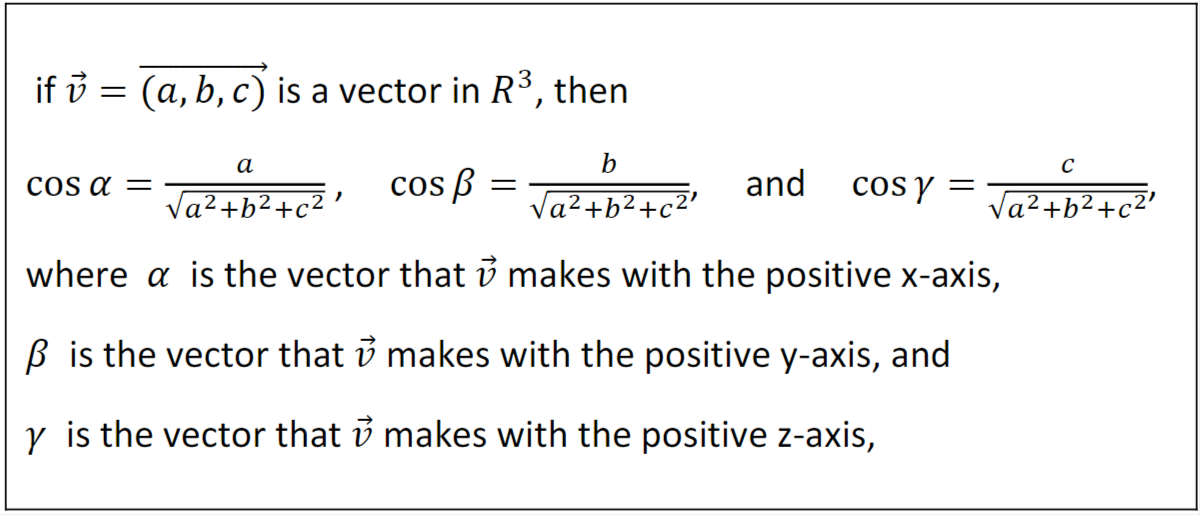
\includegraphics[width=0.7\linewidth]{imgs/image.png}
    \label{fig:enter-label}
\end{figure}
\subsubsection*{Example}
Determine the angle made by the vector $\overrightarrow{(-2,-6,3)}$ with each of the positive axes.
\subsubsection*{Solution }
\begin{align*}
    \cos \alpha = \frac{-2}{\sqrt{(-2)^2 + (-6)^2 + 3^2}} = -\frac{2}{7} \implies \alpha \approx \cos^{-1}\left(-\frac{2}{7}\right) \approx 106.6^{\circ}\\
    \cos \beta = \frac{-6}{\sqrt{(-2)^2 + (-6)^2 + 3^2}} = -\frac{6}{7} \implies \beta \approx \cos^{-1}\left(-\frac{6}{7}\right) \approx 151.9^{\circ}\\
    \cos \gamma = \frac{3}{\sqrt{(-2)^2 + (-6)^2 + 3^2}} = \frac{3}{7} \implies \gamma \approx \cos^{-1}\left(\frac{3}{7}\right) \approx 64.6^{\circ}
\end{align*}

\newpage 
\subsection{Cross Product(Aka the Vector Product)}
If you are given two non-zero vectors in $R^2$, it is not necessarily possible to find a vector perpendicular to both of the given vectors.

For example, consider the two vectors at the right.\\

However, it is a different story in $R^3 \ldots$\\

If you are given any two non-zero vectors in $R^3$, it is possible to find a third vector perpendicular to both of the given vectors. One way of doing this is called the cross-product.\\

The reason that it is always possible in $R^3$ is because you have a third dimension. (Think of the perpendicular vector as coming out of the page, or going into the page). Perhaps it's helpful to think of the $x$ and $y$ and $z$ axes. That third dimension provides us with an opportunity to find a vector perpendicular to each of the given vectors.\\
\begin{tcolorbox}[enhanced,frame style image=blueshade.png,
  opacityback=0.75,opacitybacktitle=0.25,
  colback=blue!5!white,colframe=blue!75!black] 
Cross Product of Two Vectors in $R^3$\\
To determine a vector perpendicular to each of two different vectors in $R^3$, we use the cross product.
Suppose $\vec{a}=\overrightarrow{\left(a_1, a_2, a_3\right)}$ and $\vec{b}=\overrightarrow{\left(b_1, b_2, b_3\right)}$. say that $\vec{v}$ is the cross product of $\vec{a}$ and $\vec{b}$, and we can write this as
$$
\begin{aligned}
& \vec{v}=\vec{a} \times \vec{b} \\
& \vec{a} \times \vec{b}=\overrightarrow{\left(a_2 b_3-a_3 b_2, a_3 b_1-a_1 b_3, a_1 b_2-a_2 b_1\right)} \\
&
\end{aligned}
$$
\end{tcolorbox}
\subsubsection*{Example 1}
Show that $\vec{v}$ (from he formula above) is perpendicular to both $\vec{a}$ and $\vec{b}$.
\subsubsection*{Proof that $\vec{v}$ is perpendicular to both $\vec{a}$ and $\vec{b}$}

To show that the vector $\vec{v} = \vec{a} \times \vec{b}$ is perpendicular to both $\vec{a}$ and $\vec{b}$, we need to demonstrate that the dot products $\vec{v} \cdot \vec{a}$ and $\vec{v} \cdot \vec{b}$ are both zero.

Given:
\[
\vec{a} = (a_1, a_2, a_3)
\]
\[
\vec{b} = (b_1, b_2, b_3)
\]
\[
\vec{v} = \vec{a} \times \vec{b} = (a_2 b_3 - a_3 b_2, a_3 b_1 - a_1 b_3, a_1 b_2 - a_2 b_1)
\]

First, we compute the dot product $\vec{v} \cdot \vec{a}$:
\[
\vec{v} \cdot \vec{a} = (a_2 b_3 - a_3 b_2) a_1 + (a_3 b_1 - a_1 b_3) a_2 + (a_1 b_2 - a_2 b_1) a_3
\]

Expanding this:
\[
\vec{v} \cdot \vec{a} = a_1 a_2 b_3 - a_1 a_3 b_2 + a_2 a_3 b_1 - a_1 a_2 b_3 + a_3 a_1 b_2 - a_2 a_3 b_1
\]

Notice that each term has a corresponding negative term that cancels it out:
\[
\vec{v} \cdot \vec{a} = (a_1 a_2 b_3 - a_1 a_2 b_3) + (a_2 a_3 b_1 - a_2 a_3 b_1) + (a_3 a_1 b_2 - a_3 a_1 b_2) = 0
\]

Thus:
\[
\vec{v} \cdot \vec{a} = 0
\]

Now, we compute the dot product $\vec{v} \cdot \vec{b}$:
\[
\vec{v} \cdot \vec{b} = (a_2 b_3 - a_3 b_2) b_1 + (a_3 b_1 - a_1 b_3) b_2 + (a_1 b_2 - a_2 b_1) b_3
\]

Expanding this:
\[
\vec{v} \cdot \vec{b} = a_2 b_1 b_3 - a_3 b_1 b_2 + a_3 b_1 b_2 - a_1 b_2 b_3 + a_1 b_2 b_3 - a_2 b_1 b_3
\]

Again, notice that each term has a corresponding negative term that cancels it out:
\[
\vec{v} \cdot \vec{b} = (a_2 b_1 b_3 - a_2 b_1 b_3) + (a_3 b_1 b_2 - a_3 b_1 b_2) + (a_1 b_2 b_3 - a_1 b_2 b_3) = 0
\]

Thus:
\[
\vec{v} \cdot \vec{b} = 0
\]

Since both dot products $\vec{v} \cdot \vec{a}$ and $\vec{v} \cdot \vec{b}$ are zero, the vector $\vec{v}$ is perpendicular to both $\vec{a}$ and $\vec{b}$. This completes the proof.
\newpage 



\subsection{Applications of the Dot Product and the Cross Product } 
\subsubsection{Application 1: Work}
Suppose that $\vec{f}$ is a constant force opening on an object at O so that this force moves the object from O to A.\\
Let $\vec{s}$ be the vector from O to A, and let $s=|\overrightarrow{OA}|$ be the scalar representing the distance that the object is displaced.\\
We know from physics that work is a scalar quantity which is equal to the magnitude of the force applied to the object in the direction of the movement, times the distance moved. The distance moved is the magnitude of the displacement, $|\vec{s}|$\\
The magnitude of the force applied is $|\vec{f}|$, and the magnitude of the force applied in the direction of the displacement is $|\vec{f}|\cos\theta$\\
Work = (force in the direction of movement) $\times$ (distance traveled)\\
\begin{align*}
    W&=|\vec{f}| \costheta \times |\vec{s}|\\
    W&=|\vec{f}| |\vec{s}| \cos \theta\\
    W&=\vec{f} \cdot \vec{s}
\end{align*}
When force is measured in the Newtons and displacement is measured in metres, then work is a scalar quantity measured in Joules (J). 1N $\cdot$ m=1 J

\subsubsection*{Example}
Marianna is pulling her daughter in a toboggan and is exerting a force of 40N acting at $24^{\circ}$ to the ground. If Marianna pulls the child a distance of 100m, how much work was done?
 \subsubsection*{Solution}
 \begin{align*}
    W&=\vec{f} \times \vec{s}\\
    &|\vec{f}||\vec{s}| \cos \theta\\
    &=(40N)(100m) \cos 20^{\circ}\\
    &\approx 3654.2 J
 \end{align*}

 \subsubsection{Application 2: Area}
 The area of a parallelogram determined by the vectors $\vec{a}$ and $\vec{b}$ is equal to $|\vec{a} \times \vec{b}|$\\
 Since a triangle is one half of a parallelogram, therefore,\\
 the area of a triangle determined by the vectors $\vec{a}$ and $\vec{b}$ is equal to $\frac{1}{2}|\vec{a}\times \vec{b}|$
\subsubsection*{Example}
 Determine the area of the parallelogram determined by the vectors $\vec{a}=\overrightarrow{(4,-7,5)}$ and $\vec{b}=\overrightarrow{(-1,0,2)}$
 \subsubsection*{Solution}
The area of the parallelogram defined by the vectors $\vec{a} = \overrightarrow{(4, -7, 5)}$ and $\vec{b} = \overrightarrow{(-1, 0, 2)}$, we need to use the cross product of the two vectors. The magnitude of the cross product gives the area of the parallelogram.

First, compute the cross product $\vec{a} \times \vec{b}$.

\[
\vec{a} \times \vec{b} = \begin{vmatrix}
\mathbf{i} & \mathbf{j} & \mathbf{k} \\
4 & -7 & 5 \\
-1 & 0 & 2
\end{vmatrix}
\]

The determinant can be expanded as follows:

\[
\vec{a} \times \vec{b} = \mathbf{i} \left((-7)(2) - (5)(0)\right) - \mathbf{j} \left((4)(2) - (5)(-1)\right) + \mathbf{k} \left((4)(0) - (-7)(-1)\right)
\]

\[
\vec{a} \times \vec{b} = \mathbf{i} (-14) - \mathbf{j} (8 + 5) + \mathbf{k} (0 - 7)
\]

\[
\vec{a} \times \vec{b} = -14\mathbf{i} - 13\mathbf{j} - 7\mathbf{k}
\]

So the cross product is:

\[
\vec{a} \times \vec{b} = \overrightarrow{(-14, -13, -7)}
\]

The magnitude of this vector is given by:

\[
|\vec{a} \times \vec{b}| = \sqrt{(-14)^2 + (-13)^2 + (-7)^2}
\]

\[
|\vec{a} \times \vec{b}| = \sqrt{196 + 169 + 49}
\]

\[
|\vec{a} \times \vec{b}| = \sqrt{414} 3\sqrt{46}
\]

So, the area of the parallelogram is $3\sqrt{46}$ square units.

 \subsubsection{Application 3: Torque}
 Torque is the running effect(twisting effect) of a force about a point.
 \begin{center}
     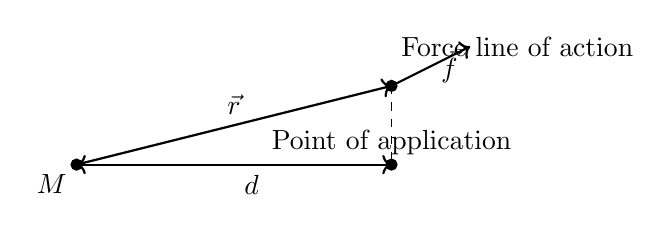
\begin{tikzpicture}
    % Define the points
    \coordinate (M) at (0,0);
    \coordinate (A) at (4,1);
    \coordinate (B) at (4,0);
    \coordinate (F) at (4,1.5);
    
    % Draw the vectors
    \draw[->, thick] (M) -- (A) node[midway, above] {$\vec{r}$};
    \draw[->, thick] (A) -- ++(1,0.5) node[midway, right] {$\vec{f}$};
    \draw[dashed] (A) -- (B);
    \draw[<->, thick] (M) -- (B) node[midway, below right] {$d$};

    % Draw the points
    \filldraw (M) circle (2pt) node[below left] {$M$};
    \filldraw (A) circle (2pt);
    \filldraw (B) circle (2pt);

    % Labels
    \node[above] at (B) {Point of application};
    \node[right] at (F) {Force line of action};

\end{tikzpicture}
 \end{center}

 In the diagram shown, the torque of the force $\vec{f}$ about the point \textit{M} is defined to be the vector $\vec{r} \times \vec{f}$. The magnitude of the torque is the product of the magnitude of the force (i,e $|\vec{f}|$) and the distance d.\\
 The force $\vec{f}$ is measured in Newtons, and the distance d is measured in metres, so the unit of magnitude for torque is Newton metres, or Jouls(J), which is the same unit that work is measured in.

 \subsubsection*{Example}
 A 20N force is applied at the end of a wrench that is 40cm in length. The force is applied at angle of $60^{\circ}$ to the wrench. Calculate the magnitude of the torque about the point of rotation M.

 \subsubsection*{Solution}
 \begin{align*}
     Torque &= |\vec{r}\times \vec{f}|\\
     &=|\vec{r}||\vec{f}| \sin \theta\\
     &=(40cm)(20N)\sin 60^{\circ}\\
     &=(0.4m)(20N)\left(\frac{\sqrt{3}}{2}\right)\\
     &=6.93 J
 \end{align*}
 \end{document}